%OBAL
\thispagestyle{empty}
\begin{center}
  \textsc{ 
    {\Large \school\\ \faculty}
    \vfill
    {\LARGE \title}\\ \vspace{0.5cm}
    {\large \thesis}
  }
\end{center}
\vfill

\begin{flushleft}
  \year\\
  \hspace{0.5cm} \author
\end{flushleft}


%TITULNY LIST
\thispagestyle{empty}
\begin{center}
  \textsc{ 
    {\Large \school\\ \faculty}
    \vfill
    {\LARGE \title}\\ \vspace{0.5cm}
    {\large \thesis}
  }
\end{center}
\vfill

\begin{flushleft}
  \begin{tabular}{@{}ll}
    Study programme: & \studyprogramme \\
    Study field: & \studyfield \\
	  Department: & \department \\
    Supervisor: & \supervisor
  \end{tabular}
  \vspace{1cm}

  \placeandyear\\
  \hspace{0.5cm} \author
\end{flushleft}



\shorthandoff{-} %docasne deaktivuje znak '-' v balicku babel
%ZADANIE EN
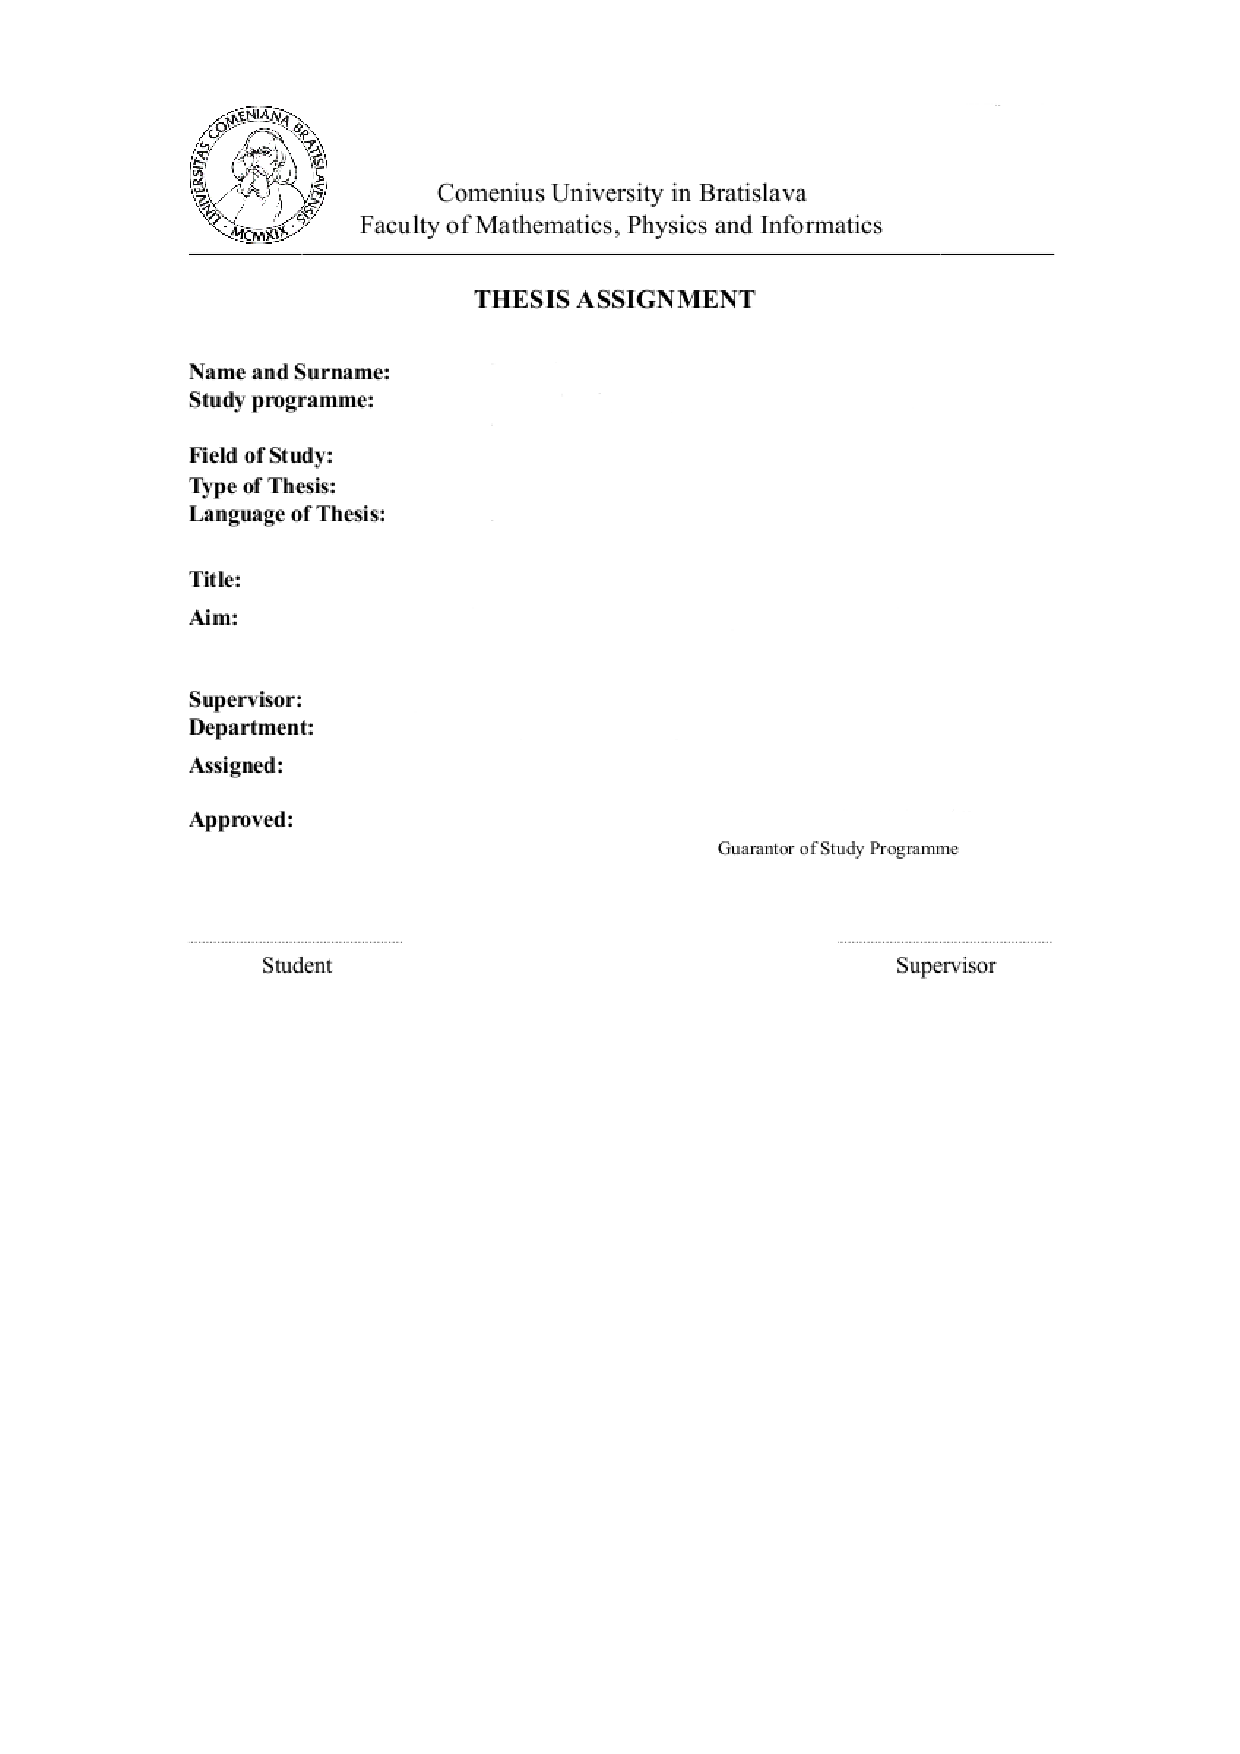
\includepdf[pages=-]{frontmatter/assignment.pdf}
%ZADANIE SK
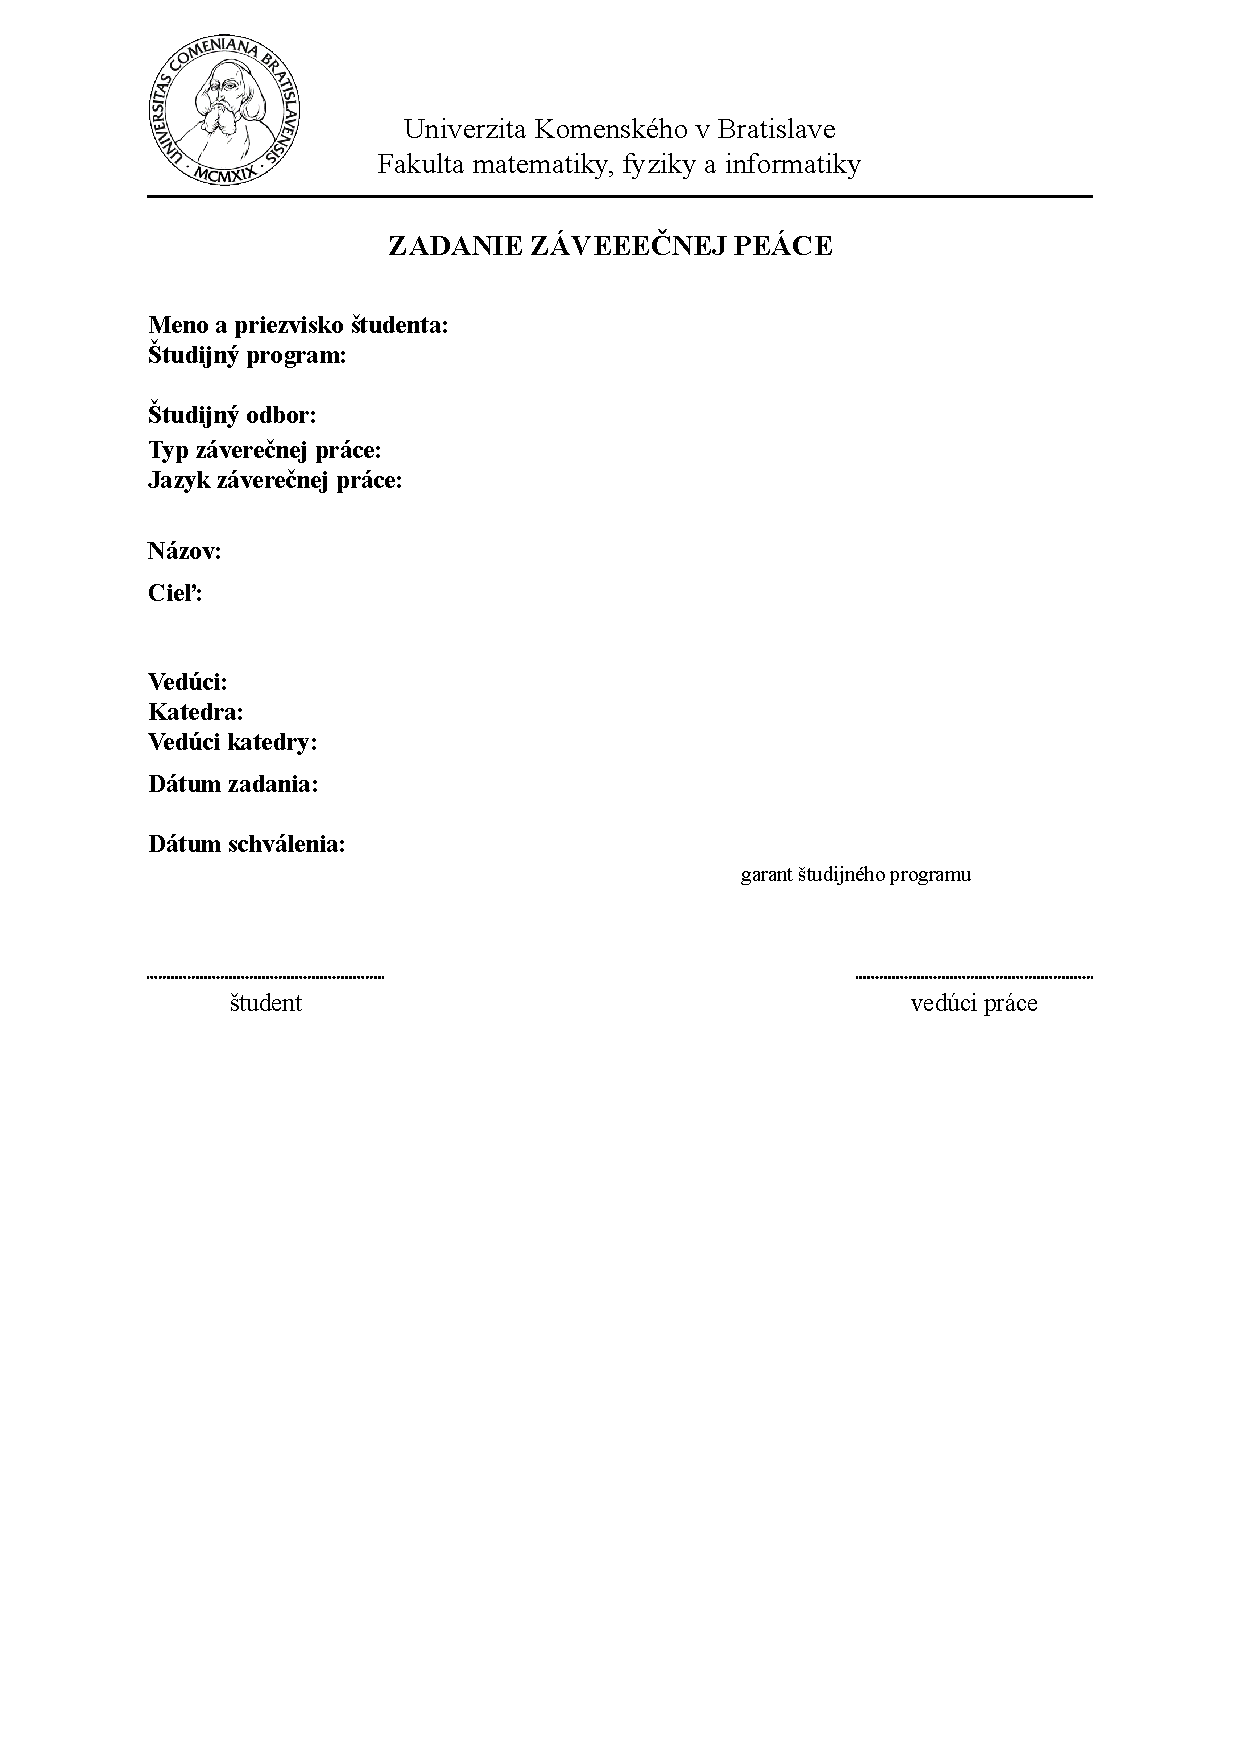
\includepdf[pages=-]{frontmatter/zadanie.pdf}
\shorthandon{-}

%PODAKOVANIE
\chapter*{Acknowledgement}
\vfil
I would like to express gratitude to my supervisor \supervisor for his help and advices by writing of this thesis. I would also like to thank my family and friends for their support during my studies.


%ABSTRAKT SK
\selectlanguage{slovak}
\chapter*{Abstrakt} 
ToDo: Abstrakt
\\
\\
\textbf{\textsc{Keywords:}} transformácie jazykov, popisná zložitosť, a-prekladač


%ABSTRAKT EN
\selectlanguage{english}
\chapter*{Abstract}
ToDo: Abstract
\\
\\
\textbf{\textsc{Keywords:}} language transformations, descriptional complexity, a-transducer


%OBSAH
\tableofcontents

%ZOZNAM ILUSTRACII
%\listoffigures
